\begin{frame}{Définition}
    Utilise les possibilités techniques du format numérique afin d’apporter un enrichissement, autant au contenu qu’à la mise en forme de l’ouvrage imprimé qu’il vient compléter. \\
    
    \textrightarrow{} Ajouter une plus-value au livre.\\
    \vspace{2em}

Problème: développement très coûteux et difficile à faire tenir dans le temps.
\end{frame}

\begin{frame}{Édition augmentée en ligne - Format WEB (HTML/XML)}
    \centering
    
\includegraphics[width=.30\textwidth]{Images/qr_code_parcours-num.png}
    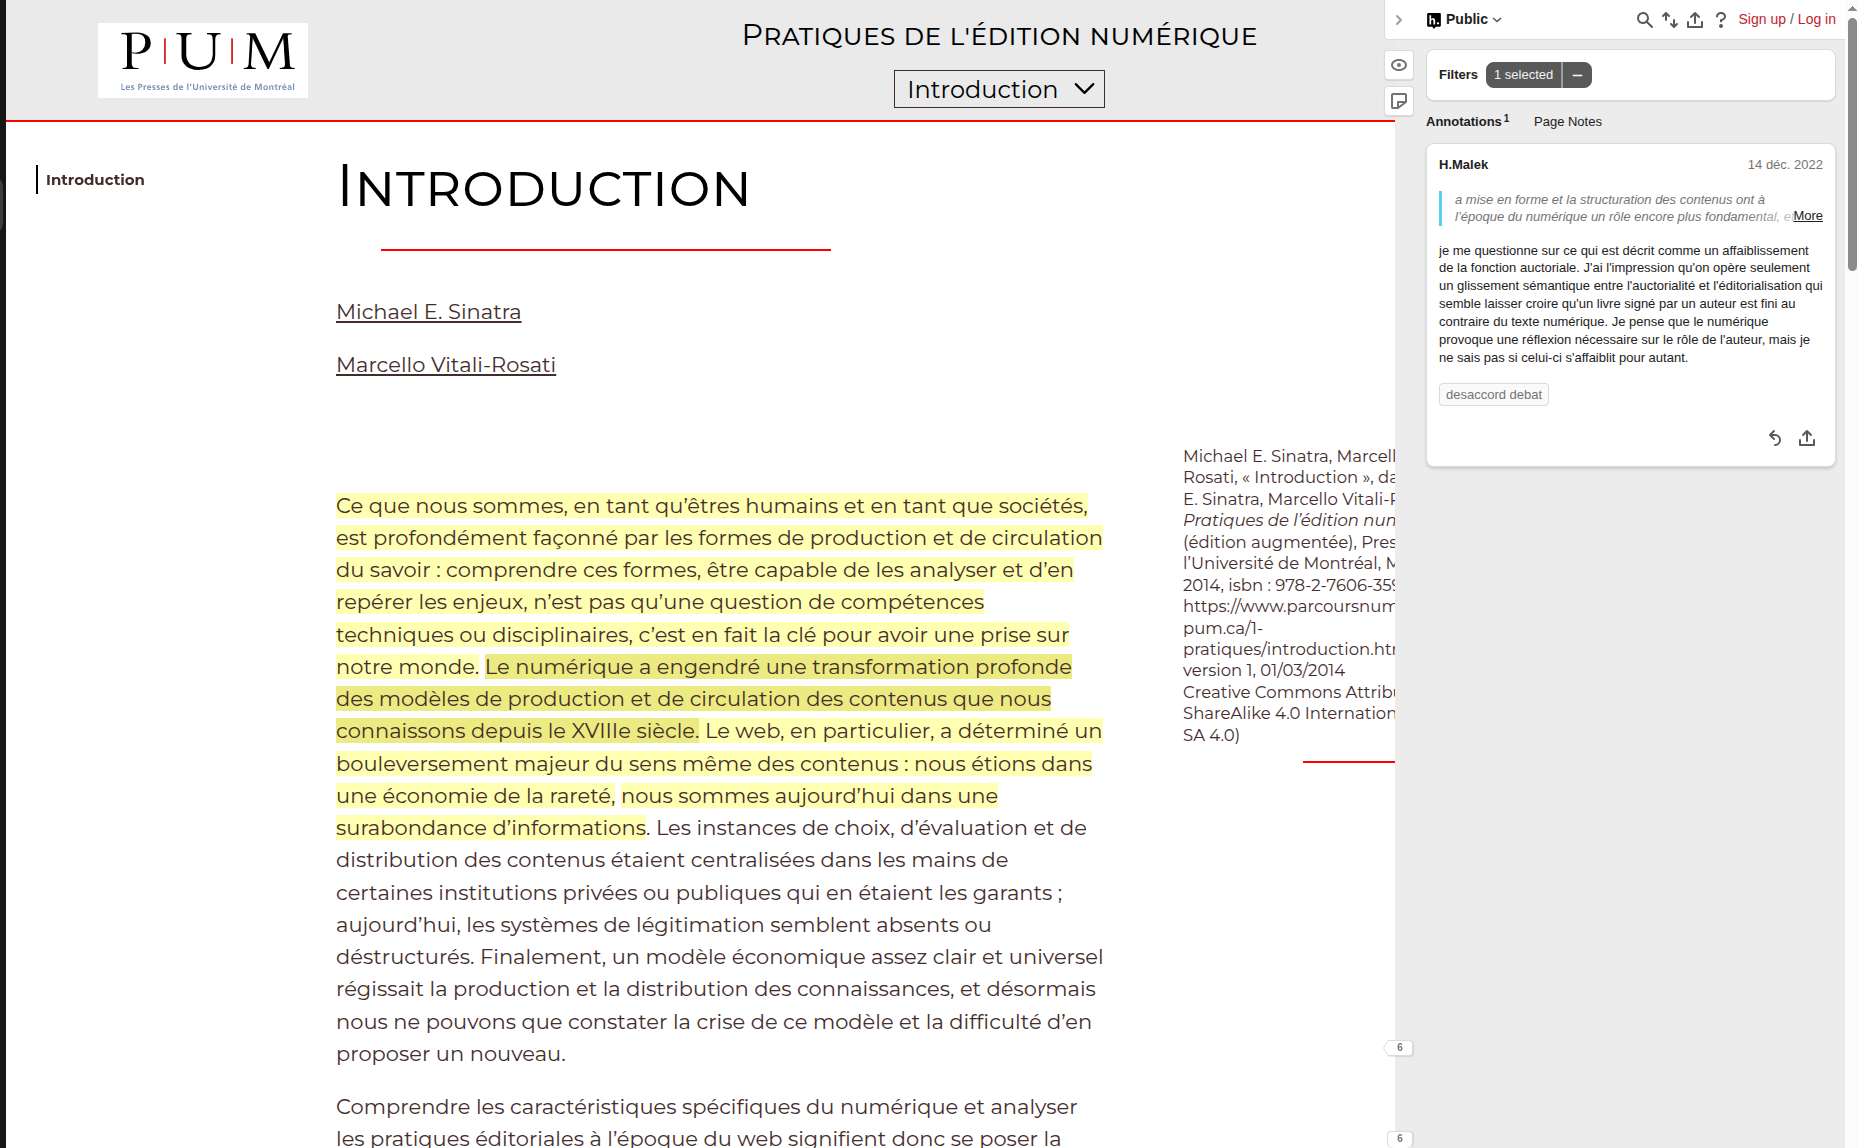
\includegraphics[width=.60\textwidth]{Images/parcoursnum-edition-augmentee.png}
\end{frame}

\begin{frame}{Édition enrichie via un dispositif transmédia (lecture délocalisée sur un appareil)}
    \begin{columns}[T,onlytextwidth]
        \column{0.50\linewidth}
        \small
        \begin{itemize}
            \item Contenu supplémentaire à l’histoire : sons, images animées en réalité augmentée qui se superposent aux pages du livre, etc.
            \item Délocalisation vers un appareil : ipad, iphone. 
            \item Problème du format de développement : 2 grosses entreprises non interopérables.
            \item Histoires animées

        \end{itemize}

        \column{0.50\linewidth}
        \centering
        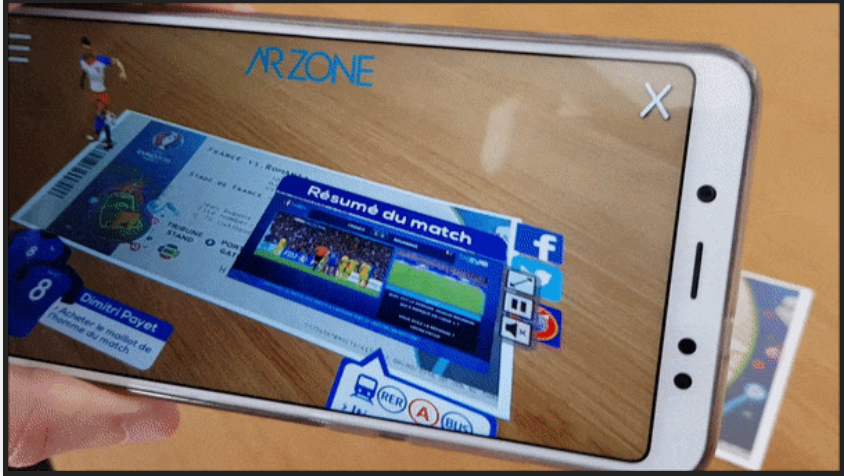
\includegraphics[width=.90\columnwidth]{Images/edition_enrichie.png}
    \end{columns}
\end{frame}